\documentclass[a4paper,11pt]{article}

\usepackage{amsmath}
\usepackage[pdftex]{graphicx}

\usepackage[english,greek]{babel}

\usepackage{lmodern}

\usepackage{listings}

\lstset{
  basicstyle=\ttfamily,
  columns=fullflexible,
  frame=single,
  breaklines=true
}

% Αφαίρεσε (Εισήγαγε) την παρακάτω γραμμή σε σχόλιο αν ο επεξεργαστής κειμένου (δεν) χρησιμοποιεί κωδικοποίηση Unicode για Ελληνικά
\usepackage[utf8x]{inputenc}

% Αφαίρεσε (Εισήγαγε) την παρακάτω γραμμή σε σχόλιο αν ο επεξεργαστής κειμένου (δεν) χρησιμοποιεί κωδικοποίηση iso-8859-7 για Ελληνικά
%\usepackage[iso-8859-7]{inputenc}

%Δημιουργία συντομεύσεων για αλλαγή γραφής σε Ελληνικά/Αγγλικά
\newcommand{\lt}{\latintext}
\newcommand{\gt}{\greektext}

\title{1η Υποχρεωτική Εργασία \\ Στο Μάθημα της Αριθμητικής Ανάλυσης: \\ Άσκηση 3}
\author{Όνοματεπώνυμο: Μπαρακλιλής Ιωάννης  \\  ΑΕΜ: 3685}
\date{16 Δεκεμβρίου 2020}

\begin{document}

\maketitle

\section*{Ζητούμενο 1: Λύση του συστήματος {\lt Ax = b}}
Ζητείται ο προγραμματισμός μιας συνάρτησης η οποία θα παίρνει σαν είσοδο τον πίνακα \textbf{\lt A} και το διάνυσμα \textbf{\lt b} του γραμμικού συστήματος \textbf{\lt Ax = b} και θα επιστρέφει σαν έξοδο το διάνυσμα των αγνώστων \textbf{\lt x}, χρησιμοποιώντας την μέθοδο επίλυσης γραμμικών συστημάτων \textbf{\lt PA = LU}.\\
Αυτό υλοποιείται στην γλώσσα {\lt python} (3.7) στο αρχείο {\lt a\textunderscore PA\textunderscore LU.py} το οποίο φαίνεται παρακάτω:

\lt
\lstinputlisting[language=Python]{a_PA_LU.py}
\gt

Στον παραπάνω κώδικα:\\
Αρχικά ορίζω τις βοηθητικές συναρτήσεις {\lt swap\textunderscore rows} που δέχεται ως παραμέτρους έναν πίνακα και δύο ακέραιους και ως λειτουργία έχει να αντιμεταθέτει άμεσα ({\lt in place}) τις γραμμές του πίνακα τις οποίες προσδιορίζουν οι παράμετροι.\\
Επίσης, ορίζεται η συνάρτηση {\lt pivot\textunderscore matrix} η οποία δέχεται ως παραμέτρους έναν πίνακα, έναν ακέραιο που προσδιορίζει την θέση ενός στοιχείου της διαγωνίου και έναν ακόμη πίνακα {\lt P} που προσδιορίζει τον πίνακα αντιμεταθέσεων και ως λειτουργία του έχει να βρίσκει το (απολύτως) μέγιστο στοιχείο της στήλης της διαγωνίου (απο την διαγώνιο και κάτω) και να αντιμεταθέτει την γραμμή με το μέγιστο με την γραμμή του στοιχείου της διαγωνίου ενώ παράλληλα ενημερώνει τον πίνακα αντιμεταθέσεων που δέχτηκε ως παράμετρο.\\
Στην συνέχεια, ορίζω την βοηθητική συνάρτηση {\lt matrix\textunderscore vector\textunderscore multiplication} που δέχεται ως παραμέτρους έναν πίνακα και ένα διάνυσμα (πίνακα στήλη) και επιστρέφει το γινόμενο του πίνακα με το διάνυσμα.\\

Μετά, ορίζω την συνάρτηση {\lt PLU} η οποία δέχεται ως παράμετρο έναν πίνακα A και επιστρέφει τους πίνακες {\lt P, L, U} που αποτελούν την παραγοντοποίηση {\lt PA = LU} του πίνακα Α.
\par
Αναλυτικά:\\
Ορίζω τους πίνακες {\lt P, U} και στην συνέχεια αντιγράφω τα περιεχόμενα του πίνακα Α στον {\lt U} ενώ παράλληλα εισάγω 0 σε κάθε στοιχείο του πίνακα {\lt P} (ο οποίος θα έχει τελικά ίδιες διαστάσεις με τον πίνακα Α). Ακολούθως, εισάγω 1 στα διαγώνια στοιχεία του πίνακα {\lt P}.\\
Στην συνέχεια, για κάθε γραμμή του πίνακα {\lt U} (εκτός της τελευταίας που παραλείπεται γιατί δεν έχει στοιχεία <<απο κάτω>>): αντιμεταθέτω την γραμμή με εκείνη της οποίας το διαγώνιο (οδηγό) στοιχείο είναι απολύτως μεγαλύτερο απο αυτά που βρίσκονται απο κάτω του στοιχείο (ταυτόχρονα ενημερώνεται και ο πίνακας αντιμεταθέσεων {\lt P}). Μετά, για κάθε γραμμή που ακολουθεί αποθηκεύω τον συντελεστή, με τον οποίο η αφαίρεση της γραμμής του οδηγού στοιχείου πολλαπλασιασμένη με τον συντελεστή με την τρέχουσα γραμμή θα <<άφηνε>> το στοιχείο της τρέχουσας γραμμής και στήλης οδηγού στοιχείου ως 0, στο στοιχείο που θα γίνονταν 0 (ώστε να μην σπαταληθεί χώρος στο να αποθηκευτούν οι συντελεστές) και αφαιρώ την υπόλοιπη γραμμή με το γινόμενο του συντελεστή αυτού επι της γραμμής του οδηγού στοιχείου. Μετά απο το τέλος αυτής της διαδικασίας, η παραγοντοποίηση {\lt PA = LU} έχει τελειώσει και απομένει να οριστούν ξεκάθαρα οι επιμέρους πίνακες {\lt L, U}.\\
Ακολούθως, δημιουργώ έναν πίνακα {\lt L} ίδου μεγέθους με τον πίνακα {\lt U} με κάθε στοιχείο του 0 και εισάγω 1 σε κάθε στοιχείο της διαγωνίου του.\\
Τελικά, εισάγω κάθε στοιχείο του πίνακα {\lt U} κάτω της διαγωνίου στην αντίστοιχη θέση του πίνακα {\lt L} και θέτω αυτό το στοιχείο του {\lt U} σε 0.\\
Η διαδικασία έχει τελειώσει, επιστρέφω τους αντίστοιχους πίνακες {\lt P, L, U}.\\

Τέλος, ορίζω την συνάρτηση {\lt solve\textunderscore system} που δέχεται ως παράμετρο έναν πίνακα συντελεστών A, και ένα διάνυσμα σταθερών {\lt b} και επιστρέφει διάνυσμα λύσεων του συστήματος χρησιμοποιώντας την μέθοδο {\lt PA = LU}.
\par
Αναλυτικά:\\
Χρησιμοποιώ την συνάρτηση {\lt PLA} που ορίστηκε παραπάνω και αποθηκεύω τα αποτελέσματα στους αντίστοιχους πίνακες, ενώ ορίζω τον πίνακα {\lt Pb} ο οποίος αποθηκεύει το γινόμενο του πίνακα {\lt P} με το διάνυσμα (πίνακα στήλη) {\lt b}.\\
Μετά, ορίζω το διάνυσμα {\lt y} και λύνω το σύστημα {\lt Ly = Pb}, του οποίου τα αποτελέσματα αποθηκεύονται στο διάνυσμα {\lt y}.\\
Τελικά, ορίζω το διάνυσμα {\lt x} και λύνω το σύστημα {\lt Ux = y} του οποίου τα αποτελέσματα αποθηκεύονται στο διάνυσμα {\lt x}, το οποίο επιστρέφω έχοντας μόλις λύσει το σύστημα {\lt Ax = b}.\\

\par
Για την λύση ενός συστήματος αρκεί κάποιος να εκτελέσει την συνάρτηση {\lt solve\textunderscore system} με τις κατάλληλες παραμέτρους.

\section*{Ζητούμενο 2: Αποσύνθεση {\lt Cholesky}}
Ζητείται ο προγραμματισμός μιας συνάρτησης που δέχεται σαν είσοδο έναν συμμετρικό και θετικά ορισμένο πίνακα A και επιστρέφει έναν κάτω τριγωνικό πίνακα {\lt L} που αποτελεί την αποσύνθεση {\lt Cholesky} του πίνακα A.

Αυτό υλοποιείται στην γλώσσα {\lt python} στο αρχείο {\lt b\textunderscore Cholesky.py} το οποίο φαίνεται παρακάτω:

\lt
\lstinputlisting[language=Python]{b_Cholesky.py}
\gt

Στον παραπάνω κώδικα:\\
Αρχικά, ορίζεται η βοηθητική συνάρτηση {\lt matrix\textunderscore multiplication} που δέχεται ως παραμέτρους δύο πίνακες και επιστρέφει το γινόμενο τους.\\
Μετά, ορίζεται η συνάρτηση {\lt cholesky\textunderscore update\textunderscore submatrix} η οποία δέχεται ως παραμέτρους έναν πίνακα και έναν ακέραιο που αντιστοιχεί στην θέση ενος διαγωνίου στοιχείου και έχει ως λειτουργία να <<προετοιμάσει>> τον πίνακα για το επόμενο βήμα του αλγορίθμου. Η αναλυτική εξήγηση της λειτουργίας του θα γίνει παρακάτω, μαζί με την εξήγηση της συνάρτησης {\lt cholesky\textunderscore core} που την χρησιμοποιεί.\\
Ακολούθως ορίζεται η αναδρομική συνάρτηση {\lt cholesky\textunderscore core} η οποία δέχεται ως παραμέτρους έναν πίνακα και έναν ακέραιο που αντιστοιχεί στην θέση ενος διαγωνίου στοιχείου.\\
\par
Αναλυτικά:\\
Αρχικά, ελέγχεται άν η θέση του διαγώνιου στοιχείου του ορίσματος είναι <<εκτός>> του πίνακα (ο ακέραιος του ορίσματος είναι μεγαλύτερος απο το μέγεθος του πίνακα) και αν ναί, επιστρέφεται ο πίνακας του ορίσματος καθώς έχει τελειώσει η διαδικασία της αποσύνθεσης  και έτσι τερματίζεται η συνάρτηση.\\
Στην συνέχεια το στοιχείο της διαγωνίου (αυτό με θέση του ορίσματος) αντικαθίσταται με την ρίζα του στοιχείου που βρίσκονταν πρίν σε αυτή την θέση και κάθε ένα απο τα υπόλοιπα στοιχεία της στήλης κάτω απο το στοιχείο της διαγωνίου διαιρείται με το νέο στοιχείο της διαγωνίου. Παράλληλα, κάθε στοιχείο της υπόλοιπης γραμμής δεξιά του στοιχείου της διαγωνίου τίθεται σε 0.\\
Στην συνέχεια ο πίνακας ενημερώνεται για το επόμενο βήμα του αλγορίθμου καλώντας την συνάρτηση {\lt cholesky\textunderscore update\textunderscore submatrix} με παραμέτρους τον πίνακα του ορίσματος και το τρέχον στοιχείο διαγωνίου. Έτσι, θα ενημερωθεί ο υποπίνακας ο οποίος έχει ως πρώτο στοιχείο το επόμενο στοιχείο της διαγωνίου.\\
Τελικά, επιστρέφεται ο πίνακας που θα επιστρέψει η αναδρομική κλήση της τρέχουσας συνάρτησης με παραμέτρους τον πίνακα του ορίσματος και το επόμενο στοιχείο της διαγωνίου. Έτσι, ο αλγόριθμος θα τελειώσει όταν γίνει επεξεργασία κάθε διαγώνιου στοιχείου, στήλης και υποπίνακα.\\

\par
Εδώ είναι το σημείο όπου θα εξηγηθεί αναλυτικά η λειτουργία της συνάρτησης {\lt cholesky\textunderscore update\textunderscore submatrix}:\\
Αρχικά, ορίζονται οι δύο πίνακες {\lt rest\textunderscore of\textunderscore column} και {\lt rest\textunderscore of\textunderscore column\textunderscore transpose} (είναι πίνακας στήλη και πίνακας γραμμή αντίστοιχα) που ο πρώτος αποθηκεύει το μέρος της στήλης του πίνακα του ορίσματος κάτω απο το στοιχείο της διαγωνίου και ο δεύτερος αποθηκεύει το ανάστροφο του πρώτου.\\
Στην συνέχεια, αποθηκεύω τον πίνακα που προκύπτει απο τον πολλαπλασιασμό αυτών των δύο πινάκων και εκτελώ αφαίρεση αυτού του πίνακα με τον υποπίνακα του πίνακα ορίσματος που έχει ως πρώτο στοιχείο το επόμενο στοιχείο της διαγωνίου (τα στοιχεία του βρίσκονται <<κάτω>> απο την γραμμή του στοιχείου διαγωνίου και <<δεξιά>> απο την στήλη αυτού).\\

\par
Τέλος, ορίζεται η συνάρτηση {\lt cholesky}, η οποία δέχεται ως παράμετρο έναν συμμετρικό και θετικά ορισμένο πίνακα και επιστρέφει έναν κάτω τριγωνικό πίνακα {\lt L} που αποτελεί την αποσύνθεση {\lt Cholesky} του πίνακα A. Η λειτουργία του είναι να εκκινεί την συνάρτηση {\lt cholesky\textunderscore core} για το πρώτο (διαγώνιο) στοιχείο του πίνακα. Για να <<πάρει>> κάποιος την αποσύνθεση {\lt cholesky} ενός συμμετρικού και θετικά ορισμένου πίνακα αρκεί κάποιος να εκτελέσει την συνάρτηση {\lt cholesky\textunderscore core} με παράμετρο τον πίνακα.

\section*{Ζητούμενο 3: Επίλυση συστήματος με μέθοδο {\lt Gauss-Seidel}}
Ζητείται ο προγραμματισμός της μεθόδου {\lt Gauss-Seidel} και η χρησιμοποίηση της για επίλυση με ακρίβεια 4 δεκαδικών ψηφίων (ως προς την άπειρη νόρμα) το {\lt $n \times n$} αραιό σύστημα \textbf{\lt Ax = b} για {\lt $n = 10$} και {\lt $n = 10000$}, με {\lt $A(i, i) = 5, A(i + 1, i) = A(i, i + 1) = −2$} και \textbf{\lt b} $= [3, 1, 1, . . . , 1, 1, 3] ^\top $.

Αυτό υλοποιείται στην γλώσσα {\lt python} στο αρχείο {\lt c\textunderscore Gauss\textunderscore Seidel.py} το οποίο φαίνεται παρακάτω:

\lt
\lstinputlisting[language=Python]{c_Gauss_Seidel.py}
\gt

Στον παραπάνω κώδικα:\\
Αρχικά, ορίζω την βοηθητική συνάρτηση {\lt vector\textunderscore subtraction} η οποία δέχεται ως παραμέτρους δύο διανύσματα και επιστρέφει την διαφορά του πρώτου με το δεύτερο.\\
Μετά, ορίζω την βοηθητική συνάρτηση {\lt max\textunderscore norm} η οποία δέχεται ως όρισμα ένα διάνυσμα και επιστρέφει την νόρμα μεγίστου (άπειρη νόρμα) αυτού.\\
\par
Ακολούθως, ορίζεται η συνάρτηση {\lt gauss\textunderscore siedel} η οποία δέχεται ως παραμέτρους τον πίνακα συντελεστών Α, τον πίνακα σταθερών {\lt b}, μία αρχική εκτίμηση για το διάνυσμα λύσης και τα απαιτούμενα ψηφία ακρίβειας.\\
Στην συνέχεια, αντιγράφονται τα περιεχόμενα του διανύσματος της αρχικής εκτίμησης στο διάνυσμα {\lt x\textunderscore old} και αρχίζει ένας ατέρμονος βρόχος που θα τερματιστεί όταν <<πετύχω>> την επιθυμιτή ακρίβεια:
\par
Αντιγράφω τα περιεχόμενα του διανύσματος (πίνακα) εκτίμησης λύσης στην μεταβλητή {\lt x} που (θα) αποθηκεύει την νέα εκτίμηση της λύσης.\\
Για κάθε στοιχείο του διανύσματος (που βρίσκεται έστω στην θέση {\lt i}) εκτίμησης λύσης θέτω ως τιμή του την σταθερά που βρίσκεται στην αντίστοιχη θέση ({\lt i}) του πίνακα σταθερών και για κάθε στοιχείο του διανύσματος εκτίμησης λύσης εκτός του τρέχοντος αφαιρώ απο το τρέχον στοιχείο το γινόμενο του άλλου στοιχείου (που βρίσκεται έστω στην θέση {\lt j}) με το στοιχείο του πίνακα συντελεστών που βρίσκεται σε γραμμή με ίδια θέση με την θέση του τρέχοντος στοιχείου στο διάνυσμα εκτίμησης λύσης ({\lt i}) και στήλη με ίδια θέση με την θέση του άλλου στοιχείου στο διάνυσμα ({\lt j}). Μετά, διαιρώ το τρέχον στοιχείο με το στοιχείο του πίνακα συντελεστών με γραμμή και στήλη με ίδια τιμή με την θέση του τρέχοντος στοιχείου στο διάνυσμα εκτίμησης λύσης ({\lt A[i][i]}).\\
Ουσιαστικα, με το παραπάνω <<λύνω>> κάθε εξίσωση του συστήματος ως προς την μεταβλητή με ίδια θέση ως προς γραμμή και στήλη υλοποιώντας το {\lt $x_i^{(m+1)} = \dfrac{1}{a_{ii}}(b_i - \sum_{j=1}^{i-1}a_{ij}x_j^{(m+1)} - \sum_{j=i+1}^{n}a_{ij}x_j^{(m)})$} της θεωρίας.\\
Το παραπάνω εκτελεί τον αλγόριθμο του {\lt Gauss-Seidel} γιατί μετά απο κάθε επανάληψη (υπολογισμός του επόμενου <<τρέχοντος στοιχείου>>) το διάνυσμα αλλάζει εφόσον έχουμε υπολογίσει το προηγούμενο στοιχείο του διανύσματος και χρησιμοποιούμε το ίδιο διάνυσμα (πίνακα) ως αποθετήριο νέας λύσης και ως σημείο πρόσβασης παλαιότερων λύσεων.\\
Τελικα, ελέγχεται άν η νόρμα μεγίστου (απείρου) της διαφοράς του νέου και του παλιού διανύσματος είναι μικρότερη απο την ζητούμενη ακρίβεια και άν είναι επιστρέφεται η τρέχουσα εκτίμηση της λύσης. Διαφορετικά, το διάνυσμα {\lt x\textunderscore old} παίρνει την τιμή του {\lt x} και συνεχίζεται η εκτέλεση του ατέρμονου βρόχου.\\

\par
Ακολουθεί ο εκτελέσιμος κώδικας ο οποίος θα εκτελεστεί αν εκτελέσουμε το παραπάνω αρχείο ο οποίος λύνει το ζητούμενο σύστημα για {\lt n = 10} και {\lt n = 10000} ως εξής:\\
Αρχικά ορίζει την σταθερά {\lt n} σε 10 και δημιουργεί τους πίνακες Α και {\lt b} σύμφωνα με την εκφώνηση .\\
Μετά, για αρχική εκτίμηση λύσης ορίζει το διάνυσμα με 1.5 σε όλα του τα στοιχεία (πλήθους {\lt n}) και εκτελεί την συνάρτηση {\lt gauss\textunderscore siedel} για τα παραπάνω και τυπώνει τα αποτελέσματα στην οθόνη.\\
Τέλος, ακολουθεί  διαδικασία ανάλογη με το πάνω για {\lt n = 10000}.\\

\par
Άν εκτελέσουμε τον παραπάνω κώδικα θα εμφανιστεί αρχικά η λύση του συστήματος για {\lt n} = 10:\\
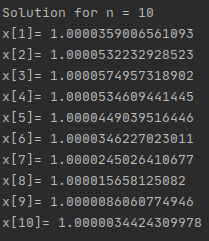
\includegraphics[width=200pt]{Exercise3/run_10.png}\\

Στο παραπάνω στιγμιότυπο εξόδου μπορούμε να δούμε ότι η λύση του συστήματος για {\lt n} = 10 είναι (με αποκοπή στα 6 δεκαδικά ψηφία) το $\textbf{\lt x} = [1.000035, 1.000053, 1.000057, 1.000053, 1.000044, 1.000034,\\ 1.000024, 1.000015, 1.000008, 1.000003]^\top$ \\

\par
Ακολουθώντας το προηγούμενο, εμφανίζεται η λύση του συστήματος για {\lt n} = 10000:\\

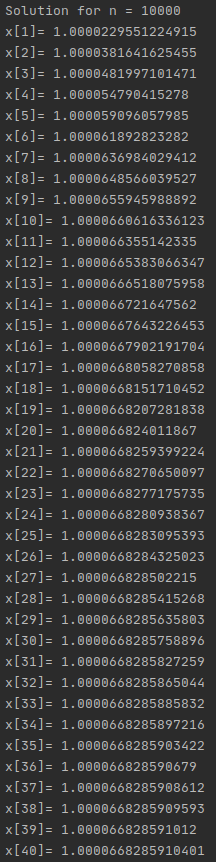
\includegraphics[width=160pt]{Exercise3/run_10000.png}\\

Στο παραπάνω στιγμιότυπο εξόδου (φαίνονται τα πρώτα 40 στοιχεία της λύσης όπου τα υπόλοιπα έχουν ανάλογες τιμές) μπορούμε να δούμε ότι η λύση του συστήματος για {\lt n} = 10000 είναι (με αποκοπή στα 6 δεκαδικά ψηφία) το $\textbf{\lt x} = [1.000022, 1.000038, ..., 1.0000025, 1.000001]^\top$\\


\end{document}
